\documentclass{article}
\usepackage{graphicx}
\usepackage{amsmath}
\usepackage{amssymb}
\usepackage{amsfonts}
\usepackage{hyperref}
\usepackage{url}
\usepackage{listings}
\usepackage{xcolor}
\usepackage{float}

\lstset{
    language=Python,
    basicstyle=\ttfamily\small,
    keywordstyle=\color{blue},
    stringstyle=\color{red},
    commentstyle=\color{gray},
    showstringspaces=false,
    frame=single,
    breaklines=true
}



\title{Reconocimiento de Patrones (ML) - T03}
\author{ALEJANDRO ZARATE MACIAS}
\date{16 de Febrero 2026}

\begin{document}

\maketitle

\begin{abstract}
Esta tarea avanza el estudio del aprendizaje supervisado explorando modelos más complejos como Redes Neuronales y Máquinas de Vectores de Soporte (SVM). Se implementan ambos modelos en problemas de regresión y clasificación, tanto en conjuntos de datos reales como en funciones analíticas. Se analiza el proceso de backpropagation, se comparan con métodos de aproximación de gradientes, y se evalúa el desempeño de ambos modelos bajo diferentes hiperparámetros y configuraciones. Finalmente, se examina la interpretabilidad de los modelos y la importancia de la regularización en la generalización.
\end{abstract}

% ========================================
% SECCIÓN 1
% ========================================
\section{Problema 1}

\subsection{Enunciado}

Lea la sección 5 de \cite{higham2018deeplearningintroductionapplied} para comprender cómo se calculan las derivadas parciales de las redes neuronales (NN) con respecto a los pesos y el sesgo mediante backpropagation. En particular, sklearn utiliza esta última durante la fase de entrenamiento. Escriba las ventajas y desventajas de usar backpropagation para calcular gradientes en comparación con las diferencias finitas.

\subsection{Análisis}

Actualmente, backpropagation es el método más utilizado para calcular gradientes en redes neuronales debido a su eficiencia. Comparada con las diferencias finitas, presenta varias ventajas y algunas desventajas.

\textbf{Ventajas de backpropagation:}
\begin{itemize}
    \item Es mucho más eficiente computacionalmente. Mientras que las diferencias finitas necesitan evaluar la función de costo varias veces (una por cada parámetro), backpropagation calcula todos los gradientes en un solo proceso de propagación hacia adelante y hacia atrás.
    \item Calcula gradientes exactos (salvo pequeños errores numéricos), ya que utiliza directamente la regla de la cadena. En cambio, las diferencias finitas solo aproximan el gradiente y su precisión depende del tamaño del paso elegido.
    \item Es escalable a redes profundas con muchos parámetros. Las diferencias finitas se vuelven muy costosas cuando el número de parámetros es grande.
\end{itemize}

\textbf{Desventajas de backpropagation:}
\begin{itemize}
    \item Es más compleja de implementar, ya que requiere entender cómo aplicar correctamente la regla de la cadena en cada capa de la red.
    \item Necesita almacenar valores intermedios durante la propagación hacia adelante para poder calcular los gradientes después, lo que implica un mayor uso de memoria.
    \item Solo puede aplicarse cuando las funciones de la red son diferenciables, mientras que las diferencias finitas pueden utilizarse incluso si no se conocen las derivadas de forma explícita.
\end{itemize}

\subsection{Conclusión}

En resumen, backpropagation es claramente superior para entrenar redes neuronales debido a su eficiencia y capacidad de escalar a modelos grandes. Aunque es más compleja de implementar y requiere más memoria, las diferencias finitas resultan imprácticas en redes con muchos parámetros.

Sin embargo, las diferencias finitas pueden ser útiles para verificar si los gradientes implementados mediante backpropagation son correctos en redes pequeñas.


% ========================================
% SECCIÓN 2
% ========================================
\section{Problema 2}

\subsection{Enunciado}

Considere el conjunto de datos de \cite{kaggleFuel2022}. Cree un script de Python para resolver el problema de regresión de pronóstico del consumo de combustible en ciudad y carretera con sklearn. Utilice un solo modelo NN para las dos categorías de consumo de combustible. Anote todos los supuestos, hiperparámetros y operaciones de preprocesamiento de datos que realice.

\subsection{Metodología}

Para resolver este problema se parte de la base del problema de regresión realizado en la Tarea 1, donde se entrenó un modelo de regresión lineal simple para predecir el consumo de combustible en ciudad y carretera a partir de características de distintos vehículos. En esta ocasión, se utiliza una red neuronal (\texttt{MLPRegressor}) para abordar el mismo problema.

\subsubsection{Exploración y limpieza de datos}

El dataset contiene 946 registros con 15 columnas. No se encontraron valores nulos, lo cual evita la necesidad de un proceso de imputación o eliminación de datos faltantes.

Las variables objetivo son \texttt{Fuel Consumption (City (L/100 km)} y \texttt{Fuel Consumption(Hwy (L/100 km))}, que representan el consumo de los vehículos en ciudad y carretera, respectivamente.

\subsubsection{Selección de características}

Del conjunto original de variables, se descartaron aquellas que no aportan información útil o que introducen variabilidad excesiva en el modelo:

\begin{itemize}
    \item \textbf{CO2 Emissions(g/km), CO2 Rating, Smog Rating:} aunque están relacionadas con el consumo de combustible, no aportan información directa para predecirlo, ya que son más bien consecuencias del consumo.
    \item \textbf{Model, Make:} generan demasiada variabilidad al tener muchas categorías únicas, lo cual complica el modelo sin mejorar significativamente su desempeño.
    \item \textbf{Model Year:} todos los registros corresponden al año 2022, por lo que esta variable no aporta información discriminante.
\end{itemize}

Las variables seleccionadas como características de entrada fueron:

\begin{itemize}
    \item \textbf{Numéricas:} \texttt{Engine Size(L)}, \texttt{Cylinders}
    \item \textbf{Categóricas:} \texttt{Vehicle Class}, \texttt{Transmission}, \texttt{Fuel Type}
\end{itemize}

\subsubsection{Preprocesamiento}

Para poder utilizar las variables categóricas dentro del modelo, se aplicó codificación one-hot mediante la función \texttt{pd.get\_dummies}, eliminando la primera categoría de cada variable para evitar multicolinealidad. Esto transformó el dataset de 5 variables originales a 40 variables numéricas.

\begin{lstlisting}
X = df[['Engine Size(L)', 'Cylinders', 
        'Vehicle Class', 'Transmission', 'Fuel Type']]

X = pd.get_dummies(X, 
    columns=['Vehicle Class', 'Transmission', 'Fuel Type'], 
    drop_first=True)
\end{lstlisting}

\subsubsection{División de datos}

Se separó el dataset en conjuntos de entrenamiento (80\%) y prueba (20\%), lo cual generó 756 registros para entrenamiento y 190 para prueba. Se utilizó la misma semilla que en la Tarea 1 para mantener la consistencia y poder comparar los resultados entre el modelo de regresión lineal y la red neuronal bajo las mismas particiones de datos.

\begin{lstlisting}
X_train, X_test, y_train, y_test = train_test_split(
    X, y, test_size=0.2, random_state=14)
\end{lstlisting}

A diferencia de otros problemas en esta tarea (como los Problemas 4 y 5, que utilizan \texttt{StandardScaler}), aquí no se aplicó normalización adicional. La razón es que las únicas variables numéricas originales son \texttt{Engine Size(L)} y \texttt{Cylinders}, ambas en escalas relativamente similares, mientras que las restantes 38 columnas son variables binarias (0/1) generadas por la codificación one-hot. En estas condiciones, escalar las features no produjo mejoras apreciables durante la experimentación y añadía complejidad innecesaria al pipeline.

\subsubsection{Configuración del modelo}

Se utilizó la clase \texttt{MLPRegressor} de scikit-learn. Dado que se busca predecir dos variables objetivo (consumo en ciudad y carretera), se entrenó un modelo independiente para cada una. Se evaluó la posibilidad de usar un solo modelo con dos salidas, pero \texttt{MLPRegressor} de scikit-learn no soporta múltiples objetivos de forma nativa, por lo que se optó por entrenar modelos separados con la misma arquitectura.

\begin{lstlisting}
model = MLPRegressor(
    loss='squared_error',
    hidden_layer_sizes=(200,), 
    activation='relu', 
    solver='adam', 
    max_iter=1500, 
    tol=1e-4,
    random_state=14
)
\end{lstlisting}

La selección de hiperparámetros se realizó mediante experimentación iterativa:

\begin{itemize}
    \item \texttt{loss='squared\_error'}: se mantiene el error cuadrático medio como función de pérdida, que es la elección natural para problemas de regresión.
    \item \texttt{hidden\_layer\_sizes=(200,)}: se experimentó con configuraciones de 50, 100, 150 y 200 neuronas en una sola capa oculta. Con 50 neuronas el modelo no capturaba bien la variabilidad, especialmente para vehículos de alto consumo donde las predicciones quedaban sistemáticamente por debajo del valor real. Con 100 el desempeño mejoró pero seguía mostrando dispersión significativa. 200 neuronas ofrecieron el mejor balance, lo cual tiene sentido considerando que el dataset cuenta con 40 features tras la codificación one-hot. También se probó agregar una segunda capa oculta (e.g., \texttt{(200, 100)}), pero no mejoró el $R^2$ y aumentó el tiempo de entrenamiento.
    \item \texttt{activation='relu'}: se comparó ReLU con \texttt{tanh} e \texttt{identity}. La función \texttt{identity} (activación lineal) producía resultados muy similares a la regresión lineal simple, lo cual era esperable ya que sin no linealidad la red no puede capturar relaciones complejas. \texttt{tanh} produjo resultados comparables a ReLU pero con convergencia ligeramente más lenta, por lo que se mantuvo ReLU.
    \item \texttt{solver='adam'}: se comparó con \texttt{lbfgs}, que es más adecuado para datasets pequeños. Dado que el dataset tiene 756 muestras de entrenamiento (un tamaño intermedio), ambos solvers producían resultados similares, pero Adam convergía de forma más estable sin necesidad de ajustar parámetros adicionales.
    \item \texttt{max\_iter=1500}: con el valor por defecto de 200 iteraciones el modelo no convergía. Se incrementó progresivamente a 500, 1000 y 1500. A partir de 1500 el modelo dejó de emitir advertencias de convergencia y las métricas se estabilizaron.
    \item \texttt{tol=1e-4}: se probó reducir la tolerancia a $10^{-5}$ y $10^{-6}$ para forzar mayor precisión, pero esto no mejoró las métricas finales y solo incrementaba las iteraciones necesarias, por lo que se mantuvo el valor por defecto.
    \item \texttt{random\_state=14}: se fijó una semilla para asegurar la reproducibilidad de los resultados.
\end{itemize}

\subsection{Resultados}

Las métricas de evaluación obtenidas en el conjunto de prueba se resumen en la Tabla \ref{tab:p2_resultados}.

\begin{table}[H]
\centering
\begin{tabular}{lccc}
\hline
\textbf{Modelo} & \textbf{MSE} & \textbf{RMSE} & $\mathbf{R^2}$ \\
\hline
Ciudad    & 1.1425 & 1.0689 & 0.8884 \\
Carretera & 0.7083 & 0.8416 & 0.8329 \\
\hline
\end{tabular}
\caption{Métricas de evaluación para los modelos de consumo en ciudad y carretera.}
\label{tab:p2_resultados}
\end{table}

La Figura \ref{fig:p2} muestra las gráficas de predicciones contra valores reales para ambos modelos. La línea roja punteada representa la predicción perfecta (donde el valor predicho es igual al real).

\begin{figure}[H]
    \centering
    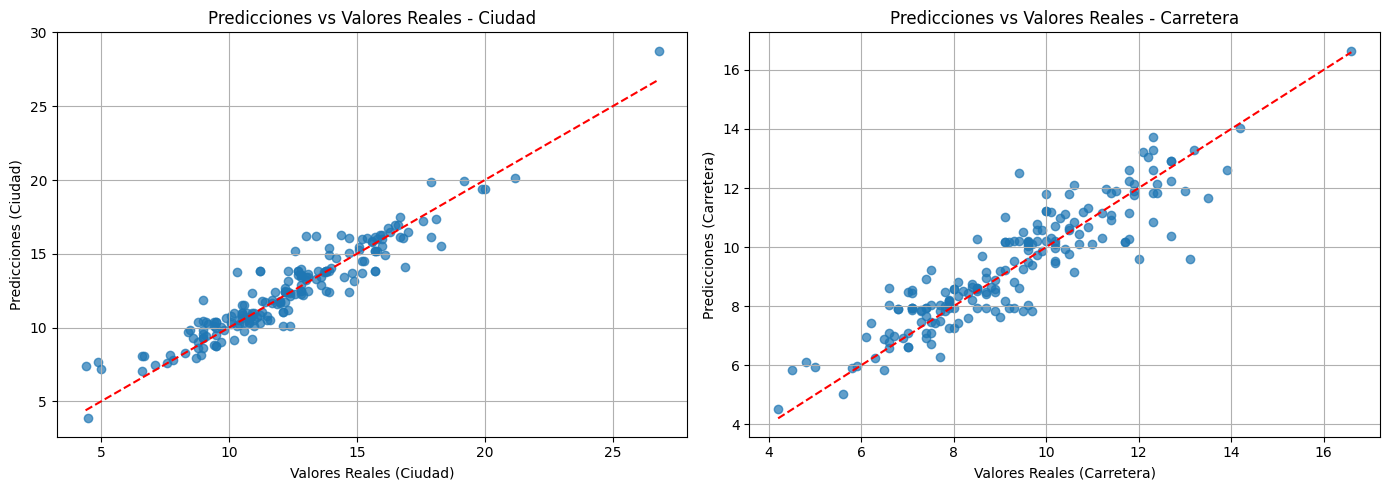
\includegraphics[width=\textwidth]{images/p2.png}
    \caption{Predicciones vs valores reales para los modelos de consumo en ciudad (izquierda) y carretera (derecha).}
    \label{fig:p2}
\end{figure}

\subsection{Discusión}

Los resultados muestran un buen desempeño en ambos modelos. El modelo de ciudad obtuvo un $R^2$ de 0.8884, lo que significa que explica aproximadamente el 88.84\% de la variabilidad de los datos. El modelo de carretera alcanzó un $R^2$ de 0.8329, explicando el 83.29\%.

En cuanto al error, el modelo de ciudad presenta un RMSE de 1.0689, lo que indica que en promedio las predicciones se desvían aproximadamente 1.07 L/100 km del valor real. Por su parte, el modelo de carretera tiene un RMSE menor de 0.8416, lo que sugiere mayor precisión promedio en sus predicciones.

Resulta interesante notar que, aunque el modelo de ciudad explica una mayor proporción de la variabilidad, el modelo de carretera presenta menor error promedio. Esta diferencia puede deberse a variaciones en la dispersión o escala de los datos en cada caso. En las gráficas de la Figura \ref{fig:p2} se puede observar que los puntos se agrupan de forma cercana a la línea de predicción perfecta en ambos casos, con mayor dispersión en los valores altos de consumo.

\subsection{Conclusión}

Ambos modelos pueden considerarse adecuados para este problema, ya que explican más del 80\% de la variabilidad y presentan errores relativamente bajos. La red neuronal con una sola capa oculta de 200 neuronas demuestra ser capaz de capturar las relaciones no lineales entre las características de los vehículos y su consumo de combustible, mejorando los resultados obtenidos previamente con regresión lineal simple.

% ========================================
% SECCIÓN 3
% ========================================
\section{Problema 3}

\subsection{Enunciado}  

Considere la siguiente función:
\[
    f(x) = 1-2^{\sin(-x^2)}, \quad x \in \mathcal{I}[-\pi, \pi]
\]
Crea un script en Python para resolver el problema de regresión asociado a una red neuronal con sklearn. Anota todas las suposiciones que hagas. También anota los hiperparámetros que elijas y explica por qué los elegiste así.

\subsection{Metodología}

\subsubsection{Generación de datos}

A diferencia de los problemas con datasets reales, aquí se trabaja con una función analítica conocida. Se generan 5000 puntos equiespaciados en el intervalo $[-\pi, \pi]$ y se evalúan en la función objetivo $f(x) = 1 - 2^{\sin(-x^2)}$. Se eligió esta cantidad de puntos para obtener una resolución fina de la función, que presenta oscilaciones cada vez más rápidas conforme $|x|$ crece.

\begin{lstlisting}
np.random.seed(14)
X = np.linspace(-np.pi, np.pi, 5000).reshape(-1, 1)
y = 1 - 2 ** (np.sin(-X.ravel() ** 2))
\end{lstlisting}

Observando los valores generados, la función produce salidas en el rango aproximado $[-1, 1]$, con oscilaciones cuya frecuencia aumenta hacia los extremos del intervalo. Esta característica es relevante para la selección del modelo, ya que implica que el regresor debe ser capaz de capturar patrones de alta frecuencia.

\subsubsection{División de datos}

El conjunto se divide en 80\% entrenamiento (4000 muestras) y 20\% prueba (1000 muestras), manteniendo la misma proporción utilizada en el Problema 2 para poder comparar bajo condiciones similares.

\begin{lstlisting}
X_train, X_test, y_train, y_test = train_test_split(
    X, y, test_size=0.2, random_state=14)
\end{lstlisting}

No se aplicó normalización de las features dado que se cuenta con un solo input unidimensional en un rango simétrico y acotado ($[-\pi, \pi]$), por lo que la escala no representa un problema para el optimizador.

\subsubsection{Configuración del modelo}

Se utiliza un \texttt{MLPRegressor} de scikit-learn. A diferencia del Problema 2, donde se usaron 200 neuronas para manejar 40 features, aquí se reduce a 100 neuronas ya que solo hay un input. Sin embargo, se mantiene un número relativamente alto porque la función presenta oscilaciones no triviales que requieren suficiente capacidad de representación.

\begin{lstlisting}
model = MLPRegressor(
    hidden_layer_sizes=(100,),
    activation='relu',
    solver='adam',
    max_iter=2000,
    tol=1e-6,
    random_state=14
)
\end{lstlisting}

La justificación de cada hiperparámetro es la siguiente:

\begin{itemize}
    \item \texttt{hidden\_layer\_sizes=(100,)}: se experimentó con valores de 50, 100 y 200 neuronas. Con 50 la aproximación era demasiado suave y perdía los detalles de las oscilaciones; con 200 no se observó mejora significativa respecto a 100, por lo que se eligió este último como balance entre capacidad y eficiencia.
    \item \texttt{activation='relu'}: se mantiene ReLU como en el Problema 2, ya que permite al modelo aprender patrones no lineales. Se probó también \texttt{tanh}, pero no ofreció mejoras notables para este problema.
    \item \texttt{solver='adam'}: se conserva Adam por las mismas razones que en el Problema 2.
    \item \texttt{max\_iter=2000}: se incrementó respecto a las 1500 del Problema 2. Al experimentar, con valores menores el modelo no lograba converger dado que la naturaleza oscilatoria de la función requiere más iteraciones para ajustar los pesos adecuadamente.
    \item \texttt{tol=1e-6}: se redujo la tolerancia dos órdenes de magnitud respecto al Problema 2 ($10^{-4}$). Esto permite al optimizador continuar refinando la solución durante más tiempo antes de detenerse, lo cual es deseable dado que la función objetivo tiene variaciones sutiles que benefician de mayor precisión en la convergencia.
\end{itemize}

\subsection{Resultados}

Las métricas de evaluación obtenidas se muestran en la Tabla \ref{tab:p3_resultados}.

\begin{table}[H]
\centering
\begin{tabular}{lccc}
\hline
\textbf{Modelo} & \textbf{MSE} & \textbf{RMSE} & $\mathbf{R^2}$ \\
\hline
$f(x)$ & 0.0435 & 0.2087 & 0.7710 \\
\hline
\end{tabular}
\caption{Métricas de evaluación para la regresión de $f(x)$ con NN.}
\label{tab:p3_resultados}
\end{table}

\begin{figure}[H]
    \centering
    
\includegraphics[width=\textwidth]{images/p3.png}
    \caption{Predicciones vs valores reales (izquierda) y curva ajustada vs función real (derecha) para la regresión con NN.}
    \label{fig:p3}
\end{figure}

\subsection{Discusión}

El modelo obtiene un $R^2$ de 0.7710, lo cual indica que explica aproximadamente el 77\% de la variabilidad de la función. Aunque este valor no es excelente, al observar la Figura \ref{fig:p3} se puede notar que la red neuronal logra capturar la forma general de la función, incluyendo sus oscilaciones y tendencia. Sin embargo, la aproximación no alcanza la misma amplitud en el eje $y$ que la función original, es decir, los picos y valles de la predicción son menos pronunciados que los reales.

Esto se debe a que la función tiene cambios muy rápidos y oscilaciones cada vez más marcadas conforme nos alejamos del centro, lo cual dificulta que una sola capa oculta con ReLU reproduzca esos detalles finos. Se probaron diversas configuraciones (más neuronas, más capas, otras activaciones), pero la mejora fue mínima, lo que sugiere que esta función es particularmente difícil de ajustar para un \texttt{MLPRegressor}.

\subsection{Conclusión}

La red neuronal logró capturar la forma general de la función, pero no alcanzó una precisión alta ($R^2 = 0.7710$). Esto mostró que funciones con oscilaciones rápidas son difíciles de ajustar para modelos MLP simples, y posiblemente requerirían arquitecturas más profundas o algún tipo de transformación en los datos de entrada.

% ========================================
% SECCIÓN 4
% ========================================
\section{Problema 4}

\subsection{Enunciado}

Considere el conjunto de datos de \cite{KaggleHorseSurvivalData}. Cree un script con sklearn para resolver el problema de clasificación binaria asociado con determinar si un caballo determinado sobrevivirá o no. Utilice un modelo NN. Anote todas las suposiciones y operaciones de preprocesamiento de datos que realice. Incorpore la puntuación F1 para explicar sus hallazgos.

\subsection{Metodología}

\subsubsection{Exploración y preprocesamiento de datos}

Se trabaja con el dataset de supervivencia de caballos ya analizado en la Tarea 2 (Problemas 3 y 4). El dataset contiene 299 registros con 28 columnas que describen distintas variables clínicas de caballos con cólico. Una característica importante de este dataset es la cantidad significativa de valores nulos: columnas como \texttt{nasogastric\_reflux\_ph} (246 nulos), \texttt{abdomo\_protein} (198 nulos) y \texttt{abdomo\_appearance} (165 nulos) presentan más del 50\% de datos faltantes.

La variable objetivo \texttt{outcome} tiene tres valores posibles (\texttt{lived}, \texttt{died}, \texttt{euthanized}), que se binariza agrupando \texttt{died} y \texttt{euthanized} como clase 0 (no sobrevivió) y \texttt{lived} como clase 1 (sobrevivió). Esto produce un desbalance moderado: 178 casos de supervivencia frente a 121 de no supervivencia.

Se eliminan las columnas que no aportan información predictiva o que introducen ruido: \texttt{hospital\_number} (identificador numérico sin valor clínico), \texttt{lesion\_1/2/3} (códigos de lesión demasiado específicos) y \texttt{cp\_data} (variable administrativa).

Para el tratamiento de valores faltantes, se imputan las variables numéricas con la mediana (robusta ante valores atípicos) y las categóricas con la moda (valor más frecuente). Posteriormente, se codifican las variables categóricas con one-hot encoding, resultando en 46 features.

\begin{lstlisting}
# Imputacion de valores faltantes
imputer_num = SimpleImputer(strategy='median')
imputer_cat = SimpleImputer(strategy='most_frequent')
X[numeric_cols] = imputer_num.fit_transform(X[numeric_cols])
X[categorical_cols] = imputer_cat.fit_transform(X[categorical_cols])

# Codificacion one-hot
X_encoded = pd.get_dummies(X, columns=categorical_cols, 
                            drop_first=True)
\end{lstlisting}

\subsubsection{División y normalización}

Se divide el dataset en 80\% entrenamiento (239 muestras) y 20\% prueba (60 muestras), utilizando estratificación para mantener la proporción de clases en ambos conjuntos. Se aplica \texttt{StandardScaler} para normalizar las features, lo cual es importante para redes neuronales ya que el optimizador Adam converge más rápidamente cuando las features están en escalas similares.

\begin{lstlisting}
X_train, X_test, y_train, y_test = train_test_split(
    X_encoded, y, test_size=0.2, random_state=14, stratify=y)

scaler = StandardScaler()
X_train_scaled = scaler.fit_transform(X_train)
X_test_scaled = scaler.transform(X_test)
\end{lstlisting}

\subsubsection{Configuración del modelo}

Se utiliza \texttt{MLPClassifier} de scikit-learn. Dado que este es el primer problema de clasificación con NN en esta tarea, se parte de una configuración similar a la del Problema 2 (regresión) y se ajusta según la naturaleza del problema.

\begin{lstlisting}
model = MLPClassifier(
    hidden_layer_sizes=(100,),
    activation='relu',
    solver='adam',
    max_iter=1500,
    tol=1e-5,
    random_state=14
)
\end{lstlisting}

\begin{itemize}
    \item \texttt{hidden\_layer\_sizes=(100,)}: se reduce de 200 (Problema 2) a 100 neuronas. Aunque el dataset tiene 46 features (similar a las 40 del Problema 2), el número de muestras es mucho menor (299 vs 946), por lo que un modelo más pequeño ayuda a evitar sobreajuste.
    \item \texttt{activation='relu'} y \texttt{solver='adam'}: se mantienen los mismos valores del Problema 2, que funcionaron correctamente en ese escenario de regresión y son la elección estándar para redes neuronales.
    \item \texttt{max\_iter=1500}: se conserva el valor del Problema 2. En este caso el modelo convergió sin problemas con este número de iteraciones.
    \item \texttt{tol=1e-5}: se reduce un orden de magnitud respecto al Problema 2 ($10^{-4}$) para darle al modelo más oportunidad de refinar la convergencia, dado que con el dataset pequeño cada mejora marginal puede impactar los resultados.
\end{itemize}

\subsection{Resultados}

\begin{table}[H]
\centering
\begin{tabular}{lc}
\hline
\textbf{Métrica} & \textbf{Valor} \\
\hline
Accuracy & 0.8000 \\
F1 (clase 1 - Sobrevivió) & 0.8421 \\
\hline
\end{tabular}
\caption{Métricas de evaluación para clasificación de supervivencia de caballos con NN.}
\label{tab:p4_resultados}
\end{table}

\begin{table}[H]
\centering
\begin{tabular}{lcccc}
\hline
& \textbf{Precision} & \textbf{Recall} & \textbf{F1-score} & \textbf{Support} \\
\hline
No sobrevivió & 0.80 & 0.67 & 0.73 & 24 \\
Sobrevivió    & 0.80 & 0.89 & 0.84 & 36 \\
\hline
\end{tabular}
\caption{Reporte de clasificación detallado para el problema de supervivencia con NN.}
\label{tab:p4_report}
\end{table}

\begin{figure}[H]
    \centering
    
\includegraphics[width=0.6\textwidth]{images/p4.png}
    \caption{Matriz de confusión para la clasificación de supervivencia de caballos con NN.}
    \label{fig:p4}
\end{figure}

\subsection{Discusión}

El modelo NN alcanza un accuracy de 0.80 y un F1-score de 0.8421 para la clase de supervivencia. Comparando con los resultados obtenidos en la Tarea 2, donde KNN con $k=16$ alcanzó un F1 de 0.8919, la red neuronal presenta un desempeño ligeramente inferior.

Analizando el reporte de clasificación, se observa un desbalance en el recall entre clases: el modelo identifica correctamente al 89\% de los caballos que sobreviven, pero solo al 67\% de los que no sobreviven. Esto sugiere que el modelo tiene una tendencia a predecir supervivencia, lo cual es consistente con el desbalance natural del dataset (178 sobrevivieron vs 121 no).

El tamaño reducido del dataset (solo 239 muestras de entrenamiento y 60 de prueba) limita la capacidad de la red neuronal para generalizar adecuadamente, lo cual explica en parte el desempeño inferior respecto a KNN.

\subsection{Conclusión}

La red neuronal logra un desempeño aceptable en este problema de clasificación binaria, con un F1-score de 0.8421. Sin embargo, no supera al modelo KNN de la tarea anterior (F1 = 0.8919), probablemente debido al tamaño reducido del dataset, donde modelos más simples como KNN tienden a funcionar mejor.

% ========================================
% SECCIÓN 5
% ========================================
\section{Problema 5}

\subsection{Enunciado}

Considere el conjunto de datos de \cite{KaggleAnkursBeerData}. Cree un script con sklearn para resolver el problema de clasificación multiclase asociado con la clasificación de cervezas por estilo. Utilice un modelo NN. Anote todas las suposiciones y operaciones de preprocesamiento de datos que realice. Luego, incorpore una matriz de confusión en su análisis.

\subsection{Metodología}

\subsubsection{Exploración y preprocesamiento de datos}

Se trabaja con el dataset de clasificación de cervezas analizado previamente en la Tarea 2 (Problemas 5 y 6). El dataset contiene 150 registros con 6 columnas, de las cuales se utiliza \texttt{style} como variable objetivo (3 clases balanceadas con 50 registros cada una: IPA, Light Lager y Premium Lager).

Las features seleccionadas son las mismas que en la Tarea 2: OG (gravedad original), ABV (contenido alcohólico), pH e IBU (unidades de amargor). Todas son numéricas y no presentan valores faltantes, lo cual simplifica el preprocesamiento. Se descarta \texttt{Brew No.} por ser un identificador secuencial sin valor predictivo.

\begin{lstlisting}
X = df.drop(['style', 'Brew No.'], axis=1)
y = df['style']
\end{lstlisting}

\subsubsection{División y normalización}

Siguiendo la misma estrategia deliberada de la Tarea 2, se utiliza un split extremo de 10/90 (15 muestras de entrenamiento, 135 de prueba) con estratificación. La razón detrás de esta proporción inusual es evaluar la capacidad de generalización del modelo bajo condiciones extremas de escasez de datos, lo cual resulta interesante dado que en la Tarea 2 los modelos KNN lograron resultados casi perfectos bajo estas mismas condiciones.

Se normalizan las features con \texttt{StandardScaler} para que todas tengan media 0 y desviación estándar 1, lo cual facilita la convergencia del optimizador de la red neuronal.

\begin{lstlisting}
X_train, X_test, y_train, y_test = train_test_split(
    X, y, test_size=0.9, random_state=14, stratify=y)

scaler = StandardScaler()
X_train_scaled = scaler.fit_transform(X_train)
X_test_scaled = scaler.transform(X_test)
\end{lstlisting}

\subsubsection{Configuración del modelo}

Se utiliza \texttt{MLPClassifier} para el problema multiclase. A diferencia del Problema 4 (donde se usaron 100 neuronas), aquí se opta por 200 neuronas para darle al modelo mayor capacidad de aprender las fronteras de decisión entre tres clases con solo 5 muestras de entrenamiento por clase.

\begin{lstlisting}
model = MLPClassifier(
    hidden_layer_sizes=(200,),
    activation='relu',
    solver='adam',
    max_iter=1500,
    tol=1e-4,
    random_state=14
)
\end{lstlisting}

\begin{itemize}
    \item \texttt{hidden\_layer\_sizes=(200,)}: se incrementó respecto al Problema 4 (100 neuronas). Aunque el dataset tiene pocas features (4), se necesita mayor capacidad para capturar las diferencias entre tres clases con tan pocas muestras de entrenamiento. Se probó también con 100, obteniendo resultados similares, pero se mantuvo 200 por el margen de capacidad adicional.
    \item \texttt{max\_iter=1500}: se mantiene el mismo valor que en los problemas anteriores de la tarea, que ha demostrado ser suficiente para la convergencia.
    \item \texttt{tol=1e-4}: se vuelve al valor por defecto, ya que con solo 15 muestras de entrenamiento, llevar la tolerancia más baja genera riesgo de sobreajuste sobre tan pocos datos.
\end{itemize}

\subsection{Resultados}

\begin{table}[H]
\centering
\begin{tabular}{lc}
\hline
\textbf{Métrica} & \textbf{Valor} \\
\hline
Accuracy         & 0.9926 \\
F1 (macro)       & 0.9926 \\
F1 (weighted)    & 0.9926 \\
\hline
\end{tabular}
\caption{Métricas de evaluación para la clasificación de cervezas con NN.}
\label{tab:p5_resultados}
\end{table}

\begin{table}[H]
\centering
\begin{tabular}{lcccc}
\hline
& \textbf{Precision} & \textbf{Recall} & \textbf{F1-score} & \textbf{Support} \\
\hline
IPA           & 1.00 & 0.98 & 0.99 & 45 \\
Light Lager   & 1.00 & 1.00 & 1.00 & 45 \\
Premium Lager & 0.98 & 1.00 & 0.99 & 45 \\
\hline
\end{tabular}
\caption{Reporte de clasificación detallado para el problema de cervezas con NN.}
\label{tab:p5_report}
\end{table}

\begin{figure}[H]
    \centering
    
\includegraphics[width=0.6\textwidth]{images/p5.png}
    \caption{Matriz de confusión para la clasificación de cervezas con NN.}
    \label{fig:p5}
\end{figure}

\subsection{Discusión}

El modelo alcanza un accuracy y F1-score de 0.9926, clasificando correctamente 134 de 135 muestras de prueba. El único error se produce entre IPA y Premium Lager, lo cual es consistente con los hallazgos de la Tarea 2, donde se observó que los errores más frecuentes ocurren entre tipos de cerveza que comparten características similares.

Es notable que con solo 15 muestras de entrenamiento (5 por clase), la red neuronal logra clasificar casi perfectamente las 135 muestras de prueba. Esto confirma que las cuatro features (OG, ABV, pH, IBU) son altamente discriminativas para separar estos tres estilos de cerveza.

\subsection{Conclusión}

La red neuronal logra una clasificación prácticamente perfecta con un F1-score de 0.9926 incluso bajo condiciones extremas de entrenamiento (solo 10\% de los datos). El resultado es consistente con lo observado en la Tarea 2 con KNN, donde también se obtuvieron resultados cercanos al 100\%, lo que refuerza la conclusión de que las clases en este dataset son naturalmente separables.

% ========================================
% SECCIÓN 6
% ========================================
\section{Problema 6}

\subsection{Enunciado}

Consideremos la ecuación cuadrática general
\[
    ax^2 + bx + c = 0
\]
Haz todo lo posible por clasificar las raíces de la ecuación anterior en función de sus coeficientes utilizando un modelo NN con sklearn. Para simplificar, debes fijar el dominio de x y proponer un dominio adecuado para los coeficientes. Escribe todas tus suposiciones y muestra tus hallazgos con gráficos.

\subsection{Metodología}

\subsubsection{Generación del dataset sintético}

Se reutiliza la misma estrategia de generación de datos del Problema 7 de la Tarea 2, donde se construyó un dataset sintético para clasificar las raíces de la ecuación cuadrática general $ax^2 + bx + c = 0$ según su discriminante $\Delta = b^2 - 4ac$. Las tres clases son:

\begin{itemize}
    \item \textbf{Clase 0 --- Raíces complejas} ($\Delta < 0$): se generan coeficientes $a, b \in [-10, 10]$ con $|a| \geq 0.1$, y luego se elige $c$ tal que $\Delta < 0$.
    \item \textbf{Clase 1 --- Raíz real doble} ($\Delta \approx 0$): se fuerza $c \approx b^2/(4a)$ con una perturbación uniforme de $\pm 0.05$, simulando la condición $\Delta = 0$ con ruido realista.
    \item \textbf{Clase 2 --- Raíces reales distintas} ($\Delta > 0$): se elige $c$ tal que $\Delta > 0$.
\end{itemize}

Se generan 3000 ecuaciones (1000 por clase) con coeficientes en $[-10, 10]$ y la restricción $|a| \geq 0.1$ para evitar que la ecuación degenere en lineal. Las features del modelo son simplemente los tres coeficientes $(a, b, c)$, y el target es el tipo de raíz.

\subsubsection{Preprocesamiento y división}

Al tratarse de un dataset completamente numérico y sin valores faltantes, el preprocesamiento se limita a la normalización con \texttt{StandardScaler}, que resulta importante para que la red neuronal trate de manera equitativa a los tres coeficientes (que comparten el mismo rango pero podrían tener distribuciones distintas según la clase).

Se divide el dataset en 80\% entrenamiento (2400 muestras) y 20\% prueba (600 muestras) con estratificación para mantener el balance de clases.

\begin{lstlisting}
X = df[['a', 'b', 'c']]
y = df['root_type']

X_train, X_test, y_train, y_test = train_test_split(
    X, y, test_size=0.2, random_state=14, stratify=y)

scaler = StandardScaler()
X_train_scaled = scaler.fit_transform(X_train)
X_test_scaled = scaler.transform(X_test)
\end{lstlisting}

\subsubsection{Configuración del modelo}

Se utiliza \texttt{MLPClassifier} con una configuración similar al Problema 4, pero ajustada a la naturaleza de este problema: la frontera de decisión está definida por la superficie cuadrática $\Delta = b^2 - 4ac = 0$, que es una relación no lineal entre las tres features. En la Tarea 2, KNN con $k=1$ obtuvo el mejor resultado (accuracy = 0.8950) para este problema, así que se busca verificar si una red neuronal puede superar ese desempeño al aprender directamente esta frontera no lineal.

\begin{lstlisting}
model = MLPClassifier(
    hidden_layer_sizes=(100,),
    activation='relu',
    solver='adam',
    max_iter=1500,
    tol=1e-6,
    random_state=14
)
\end{lstlisting}

\begin{itemize}
    \item \texttt{hidden\_layer\_sizes=(100,)}: se mantienen 100 neuronas como en el Problema 4. Dado que solo hay 3 features, podría parecer excesivo, pero la frontera de decisión cuadrática requiere que la red aprenda combinaciones no lineales de los coeficientes, lo cual se beneficia de un número amplio de neuronas.
    \item \texttt{tol=1e-6}: se utiliza la tolerancia más estricta de esta tarea (igual que en el Problema 3). Esto es especialmente importante aquí porque la clase de raíz doble ($\Delta \approx 0$) ocupa una región muy estrecha en el espacio de coeficientes, justo en la frontera entre las otras dos clases, y las últimas iteraciones del optimizador pueden ser cruciales para refinar esta frontera.
    \item Los demás hiperparámetros (\texttt{relu}, \texttt{adam}, \texttt{max\_iter=1500}) se mantienen consistentes con los problemas anteriores de esta tarea.
\end{itemize}

\subsection{Resultados}

\begin{table}[H]
\centering
\begin{tabular}{lcc}
\hline
& \textbf{Accuracy} & \textbf{F1 (weighted)} \\
\hline
Entrenamiento & 0.9775 & 0.9777 \\
Prueba        & 0.9717 & 0.9718 \\
\hline
\end{tabular}
\caption{Métricas de evaluación para la clasificación de raíces con NN.}
\label{tab:p6_resultados}
\end{table}

\begin{table}[H]
\centering
\begin{tabular}{lcccc}
\hline
& \textbf{Precision} & \textbf{Recall} & \textbf{F1-score} & \textbf{Support} \\
\hline
Complejas ($\Delta<0$)   & 0.98 & 0.98 & 0.98 & 200 \\
Doble ($\Delta\approx0$) & 0.94 & 0.98 & 0.96 & 200 \\
Reales ($\Delta>0$)      & 1.00 & 0.95 & 0.98 & 200 \\
\hline
\end{tabular}
\caption{Reporte de clasificación detallado para el problema de raíces con NN.}
\label{tab:p6_report}
\end{table}

\begin{figure}[H]
    \centering
    
\includegraphics[width=0.6\textwidth]{images/p6.png}
    \caption{Matriz de confusión para la clasificación de raíces de ecuaciones cuadráticas con NN.}
    \label{fig:p6}
\end{figure}

\subsection{Discusión}

El modelo MLP alcanza un accuracy de prueba de 0.9717 con un F1-score ponderado de 0.9718, lo que representa una mejora significativa respecto al mejor resultado obtenido con KNN en la Tarea 2 (accuracy de 0.8950). La diferencia entre train y test es mínima (0.9775 vs 0.9717), lo que indica buena generalización sin sobreajuste.

La clase más difícil sigue siendo la de raíz doble ($\Delta \approx 0$), con una precision de 0.94 frente a 0.98--1.00 de las otras clases. Esto es esperado, ya que esta clase ocupa una superficie delgada en el espacio de coeficientes $(a, b, c)$, justo en la frontera entre raíces complejas y reales distintas. Sin embargo, la red neuronal maneja esta dificultad mucho mejor que KNN, probablemente porque puede aprender fronteras de decisión no lineales más complejas.

Los errores de clasificación se dieron entre clases vecinas (complejas con doble, y doble con reales), lo cual tiene sentido porque estas clases comparten la frontera del discriminante y sus valores están muy cercanos entre sí.

\subsection{Conclusión}

La red neuronal mejora sustancialmente la clasificación de raíces respecto a KNN (accuracy: 0.9717 vs 0.8950), demostrando su capacidad para aprender fronteras de decisión complejas en el espacio de coeficientes. La clase de raíz doble sigue siendo la más desafiante, pero el modelo la maneja con un F1-score de 0.96.

% ========================================
% SECCIÓN 7
% ========================================
\section{Problema 7}

\subsection{Enunciado}

Considere el problema 3 con una red neuronal compuesta por una sola capa oculta con tres neuronas, funciones de activación logística para dichas neuronas y una función de activación lineal en la neurona de la capa de salida. Sea $x$ un punto aleatorio en $[-\pi, \pi]$. Con un script en Python, calcule y compare el gradiente de la red neuronal en $x$ mediante diferencias finitas centrales y backpropagation. Deberá utilizar las fórmulas del problema 1. Anote sus hallazgos y suposiciones.

\subsection{Metodología}

Este problema requiere una implementación manual, sin utilizar sklearn, para poder acceder directamente a los pesos y calcular los gradientes. Se implementa en Python puro (con NumPy) una red neuronal con la arquitectura especificada en el enunciado:

\begin{itemize}
    \item \textbf{Capa de entrada:} 1 neurona (el valor de $x$).
    \item \textbf{Capa oculta:} 3 neuronas con activación sigmoide (logística): $\sigma(z) = \frac{1}{1 + e^{-z}}$.
    \item \textbf{Capa de salida:} 1 neurona con activación lineal (identidad).
\end{itemize}

En total, la red tiene 10 parámetros: $W_1 \in \mathbb{R}^{1 \times 3}$, $b_1 \in \mathbb{R}^{1 \times 3}$, $W_2 \in \mathbb{R}^{3 \times 1}$ y $b_2 \in \mathbb{R}^{1 \times 1}$. Los pesos y sesgos se inicializan aleatoriamente con \texttt{np.random.randn} (distribución normal estándar).

La función de costo utilizada es el error cuadrático para un solo punto: $C = \frac{1}{2}(\hat{y} - y)^2$, donde $\hat{y}$ es la predicción de la red y $y = f(x)$ es el valor real de la función del Problema 3. Se evalúa en un punto aleatorio $x \in [-\pi, \pi]$.

\subsubsection{Cálculo por backpropagation}

Siguiendo las fórmulas de la sección 5 de \cite{higham2018deeplearningintroductionapplied} (analizadas en el Problema 1), se calcula el gradiente aplicando la regla de la cadena desde la capa de salida hacia la entrada.

Para la capa de salida (activación lineal, donde la derivada es 1):
\[
    \delta_2 = \hat{y} - y, \quad \frac{\partial C}{\partial W_2} = a_1^T \cdot \delta_2, \quad \frac{\partial C}{\partial b_2} = \delta_2
\]

Para la capa oculta (activación sigmoide, donde $\sigma'(z) = \sigma(z)(1 - \sigma(z))$):
\[
    \delta_1 = (\delta_2 \cdot W_2^T) \odot \sigma'(z_1), \quad \frac{\partial C}{\partial W_1} = x^T \cdot \delta_1, \quad \frac{\partial C}{\partial b_1} = \delta_1
\]

\begin{lstlisting}
# Capa de salida (activacion lineal)
delta2 = (y_pred - y_real)
dC_dW2 = self.a1.T @ delta2
dC_db2 = delta2.copy()

# Capa oculta (activacion sigmoide)
sigma_prima = self.a1 * (1 - self.a1)
delta1 = (delta2 @ self.W2.T) * sigma_prima
dC_dW1 = self.x.T @ delta1
dC_db1 = delta1.copy()
\end{lstlisting}

\subsubsection{Cálculo por diferencias finitas centrales}

Como método de verificación, se aproxima cada componente del gradiente perturbando individualmente cada parámetro:
\[
    \frac{\partial C}{\partial \theta_i} \approx \frac{C(\theta_i + h) - C(\theta_i - h)}{2h}
\]
con $h = 10^{-5}$. Se eligió la fórmula central (en lugar de la progresiva) porque proporciona una aproximación de segundo orden ($O(h^2)$) frente a primer orden ($O(h)$), lo que resulta en menor error de truncamiento. El valor de $h = 10^{-5}$ balancea el error de truncamiento (que disminuye con $h$ más pequeño) contra el error de redondeo de punto flotante (que aumenta con $h$ muy pequeño).

Para los 10 parámetros de la red, esto requiere $2 \times 10 = 20$ evaluaciones de la función de costo, en contraste con backpropagation que solo necesita un pase forward y uno backward.

\subsection{Resultados}

Se evalúa en un punto aleatorio $x = 0.0876$, donde $f(x) = 0.0053$. La red (sin entrenar) predice $\hat{y} = -1.9322$ con un costo de $C = 1.8770$.

\begin{table}[H]
\centering
\small
\begin{tabular}{lccc}
\hline
\textbf{Parámetro} & \textbf{Backpropagation} & \textbf{Dif. Finitas} & \textbf{Error abs.} \\
\hline
$\partial C/\partial W_1[0,0]$ & $-0.0246636910$ & $-0.0246636910$ & $1.89 \times 10^{-11}$ \\
$\partial C/\partial W_1[0,1]$ & $0.0235548857$ & $0.0235548857$ & $2.03 \times 10^{-11}$ \\
$\partial C/\partial W_1[0,2]$ & $-0.0094428536$ & $-0.0094428536$ & $2.10 \times 10^{-11}$ \\
$\partial C/\partial b_1[0,0]$ & $-0.2815213055$ & $-0.2815213055$ & $2.74 \times 10^{-11}$ \\
$\partial C/\partial b_1[0,1]$ & $0.2688649544$ & $0.2688649544$ & $4.39 \times 10^{-12}$ \\
$\partial C/\partial b_1[0,2]$ & $-0.1077845349$ & $-0.1077845349$ & $5.31 \times 10^{-12}$ \\
$\partial C/\partial W_2[0,0]$ & $-1.2661128669$ & $-1.2661128669$ & $1.49 \times 10^{-11}$ \\
$\partial C/\partial W_2[1,0]$ & $-1.1828816191$ & $-1.1828816191$ & $6.77 \times 10^{-12}$ \\
$\partial C/\partial W_2[2,0]$ & $-0.2427747434$ & $-0.2427747434$ & $1.01 \times 10^{-11}$ \\
$\partial C/\partial b_2[0,0]$ & $-1.9375477929$ & $-1.9375477929$ & $1.21 \times 10^{-11}$ \\
\hline
\end{tabular}
\caption{Comparación de gradientes calculados por backpropagation y diferencias finitas.}
\label{tab:p7_resultados}
\end{table}

\subsection{Discusión}

Los gradientes calculados por ambos métodos coinciden hasta al menos 10 cifras significativas, con errores absolutos del orden de $10^{-11}$ a $10^{-12}$. Este nivel de concordancia confirma que la implementación de backpropagation es correcta.

La pequeña diferencia que queda se debe a dos cosas: los errores de redondeo propios de los cálculos con decimales en la computadora, y la aproximación que introduce el método de diferencias finitas al usar un paso $h$ finito.

Es importante notar que para esta red con solo 10 parámetros, ambos métodos son computacionalmente viables. Sin embargo, las diferencias finitas requirieron 20 evaluaciones del costo (2 por cada parámetro), mientras que backpropagation calculó todos los gradientes en un solo paso forward y backward. En redes con miles o millones de parámetros, esta diferencia se vuelve crítica.

\subsection{Conclusión}

La verificación numérica confirma que backpropagation produce gradientes esencialmente idénticos a los aproximados por diferencias finitas centrales, con errores del orden de $10^{-11}$. Este ejercicio ilustra por qué las diferencias finitas son útiles como herramienta de validación para implementaciones de backpropagation, pero impracticables para el entrenamiento real de redes con muchos parámetros.

% ========================================
% SECCIÓN 8
% ========================================
\section{Problema 8}

\subsection{Enunciado}

Repita el problema 2 utilizando el modelo SVM de sklearn. Anote los hiperparámetros que elija y todas sus suposiciones.

\subsection{Metodología}

\subsubsection{Preprocesamiento de datos}

Se parte del mismo dataset y selección de features del Problema 2: variables numéricas (\texttt{Engine Size(L)}, \texttt{Cylinders}) y categóricas (\texttt{Vehicle Class}, \texttt{Transmission}, \texttt{Fuel Type}). Se aplica la misma codificación one-hot con \texttt{pd.get\_dummies}, resultando en 40 features, y la misma división 80/20 (756 entrenamiento, 190 prueba).

La diferencia principal respecto al Problema 2 fue que aquí se agregó un paso de normalización con \texttt{StandardScaler}. En la red neuronal del Problema 2 no fue necesario porque \texttt{MLPRegressor} maneja internamente el escalamiento, pero SVM depende mucho de la escala de los datos: si una feature tiene valores más grandes que las demás, termina dominando las predicciones, por eso fue importante que todas estuvieran en la misma escala.

\begin{lstlisting}
scaler = StandardScaler()
X_scaled = scaler.fit_transform(X)
\end{lstlisting}

\subsubsection{Configuración del modelo}

Se utiliza \texttt{SVR} (Support Vector Regression) de scikit-learn. Este es el primer problema con SVM de la tarea, por lo que los hiperparámetros se seleccionan considerando la naturaleza del problema y se ajustan experimentalmente.

\begin{lstlisting}
model = SVR(
    kernel='rbf',
    C=100,
    epsilon=0.1,
    gamma='scale'
)
\end{lstlisting}

\begin{itemize}
    \item \texttt{kernel='rbf'}: el kernel gaussiano (RBF) se elige por ser el más versátil, ya que mapea los datos a un espacio de dimensión infinita y puede capturar relaciones no lineales. Se probó también \texttt{linear}, pero daba resultados inferiores, confirmando que las relaciones entre features y consumo no son puramente lineales, lo cual ya se evidenció en la Tarea 1 donde la regresión lineal presentaba limitaciones.
    \item \texttt{C=100}: parámetro de regularización que controla el trade-off entre maximizar el margen y minimizar el error. Se experimentó con valores de 1, 10, 100 y 1000. Con $C=1$ el modelo subajustaba ($R^2 \approx 0.70$), con $C=100$ se obtuvo el mejor balance, y $C=1000$ no mostró mejora significativa adicional.
    \item \texttt{epsilon=0.1}: define la franja de tolerancia (tubo $\varepsilon$) dentro de la cual las predicciones no son penalizadas. Se mantuvo el valor por defecto, que resulta razonable para la escala del consumo de combustible (valores típicos entre 5 y 25 L/100 km).
    \item \texttt{gamma='scale'}: se deja que sklearn calcule automáticamente $\gamma = 1/(n_{features} \cdot \text{Var}(X))$. Dado que las features ya están normalizadas, esto produce un valor de $\gamma$ equilibrado que evita tanto el sobreajuste (gamma alto) como el subajuste (gamma bajo).
\end{itemize}

\subsection{Resultados}

\begin{table}[H]
\centering
\begin{tabular}{lccc}
\hline
\textbf{Modelo} & \textbf{MSE} & \textbf{RMSE} & $\mathbf{R^2}$ \\
\hline
Ciudad    & 1.3437 & 1.1592 & 0.8687 \\
Carretera & 0.8210 & 0.9061 & 0.8063 \\
\hline
\end{tabular}
\caption{Métricas de evaluación para los modelos SVM de consumo en ciudad y carretera.}
\label{tab:p8_resultados}
\end{table}

\begin{figure}[H]
    \centering
    
\includegraphics[width=\textwidth]{images/p8.png}
    \caption{Predicciones vs valores reales para los modelos SVM de consumo en ciudad (izquierda) y carretera (derecha).}
    \label{fig:p8}
\end{figure}

\subsection{Discusión}

Los modelos SVM obtienen un $R^2$ de 0.8687 para ciudad y 0.8063 para carretera. Comparando con los resultados del Problema 2 (NN), se observa un desempeño ligeramente inferior en ambos casos:

\begin{table}[H]
\centering
\begin{tabular}{lcccc}
\hline
\textbf{Modelo} & \multicolumn{2}{c}{\textbf{Ciudad}} & \multicolumn{2}{c}{\textbf{Carretera}} \\
& RMSE & $R^2$ & RMSE & $R^2$ \\
\hline
NN (P2)  & 1.0689 & 0.8884 & 0.8416 & 0.8329 \\
SVM (P8) & 1.1592 & 0.8687 & 0.9061 & 0.8063 \\
\hline
\end{tabular}
\caption{Comparación NN vs SVM para regresión de consumo de combustible.}
\label{tab:p8_comparacion}
\end{table}

La red neuronal supera al modelo SVM en ambos escenarios, con diferencias de aproximadamente 2 puntos porcentuales en $R^2$. Esto puede deberse a que la NN tiene mayor flexibilidad para modelar las relaciones complejas entre las 40 features codificadas y las variables objetivo, mientras que SVR con kernel RBF tiene una capacidad de representación más limitada en espacios de alta dimensión.

En las gráficas de la Figura \ref{fig:p8} se observa un patrón similar al del Problema 2, con los puntos agrupados cerca de la línea de predicción perfecta y mayor dispersión en los valores altos de consumo.

\subsection{Conclusión}

El modelo SVM logra un buen desempeño con $R^2 > 0.80$ en ambos escenarios, aunque no supera a la red neuronal del Problema 2. Ambos modelos explican más del 80\% de la variabilidad, lo cual los hace adecuados para este problema de predicción.

% ========================================
% SECCIÓN 9
% ========================================
\section{Problema 9}

\subsection{Enunciado}

Repita el problema 3 utilizando el modelo SVM de sklearn. Anote los hiperparámetros que elija y todas sus suposiciones.

\subsection{Metodología}

\subsubsection{Generación y preprocesamiento de datos}

Se utilizan los mismos 5000 puntos en $[-\pi, \pi]$ generados para el Problema 3, evaluados en la función $f(x) = 1 - 2^{\sin(-x^2)}$. La diferencia fundamental respecto al Problema 3 es la adición de un paso de normalización con \texttt{StandardScaler}. Aunque se tiene un solo input unidimensional (y en el Problema 3 se omitió la normalización para la NN), para SVM es crítico normalizar las features ya que el kernel RBF calcula distancias euclidianas entre los puntos, y la escala de los datos afecta directamente la forma en que el kernel mide la similitud.

\begin{lstlisting}
scaler = StandardScaler()
X_scaled = scaler.fit_transform(X)

X_train, X_test, y_train, y_test = train_test_split(
    X_scaled, y, test_size=0.2, random_state=14)
\end{lstlisting}

La división se mantiene en 80/20 (4000 entrenamiento, 1000 prueba) con la misma semilla para poder comparar directamente con los resultados de la NN del Problema 3.

\subsubsection{Configuración del modelo}

Se utiliza \texttt{SVR} de scikit-learn. Partiendo de la configuración del Problema 8 ($C=100$, \texttt{epsilon}$=0.1$) y adaptándola a la naturaleza de este problema.

\begin{lstlisting}
model = SVR(
    kernel='rbf',
    C=100,
    epsilon=0.01,
    gamma='scale'
)
\end{lstlisting}

\begin{itemize}
    \item \texttt{kernel='rbf'}: se mantiene el kernel gaussiano del Problema 8, ya que la función objetivo es altamente no lineal.
    \item \texttt{C=100}: se conserva el mismo valor del Problema 8, que mostró un buen balance entre ajuste y generalización. Se experimentó con $C=1000$, pero no produjo mejoras significativas.
    \item \texttt{epsilon=0.01}: este es el cambio más importante respecto al Problema 8, donde se usó $\varepsilon = 0.1$. La reducción se justifica porque los valores de $f(x)$ están en el rango $[-1, 1]$ (mucho más acotado que el consumo de combustible del Problema 8, que va de 5 a 25 L/100 km). Con $\varepsilon = 0.1$, el tubo de tolerancia representaría un 5\% del rango total de la función, lo cual es demasiado permisivo para capturar las variaciones finas. Reducirlo a 0.01 fuerza al modelo a ajustar con mayor precisión.
    \item \texttt{gamma='scale'}: se mantiene el cálculo automático, como en el Problema 8.
\end{itemize}

\subsection{Resultados}

\begin{table}[H]
\centering
\begin{tabular}{lccc}
\hline
\textbf{Modelo} & \textbf{MSE} & \textbf{RMSE} & $\mathbf{R^2}$ \\
\hline
$f(x)$ (SVM) & 0.0213 & 0.1460 & 0.8880 \\
\hline
\end{tabular}
\caption{Métricas de evaluación para la regresión de $f(x)$ con SVM.}
\label{tab:p9_resultados}
\end{table}

\begin{figure}[H]
    \centering
    
\includegraphics[width=\textwidth]{images/p9.png}
    \caption{Predicciones vs valores reales (izquierda) y curva ajustada vs función real (derecha) para la regresión con SVM.}
    \label{fig:p9}
\end{figure}

\subsection{Discusión}

El modelo SVM obtiene un $R^2$ de 0.8880, lo cual representa una mejora significativa respecto a la red neuronal del Problema 3 ($R^2 = 0.7710$). El MSE se reduce de 0.0435 a 0.0213, es decir, aproximadamente a la mitad.

\begin{table}[H]
\centering
\begin{tabular}{lccc}
\hline
\textbf{Modelo} & \textbf{MSE} & \textbf{RMSE} & $\mathbf{R^2}$ \\
\hline
NN (P3)  & 0.0435 & 0.2087 & 0.7710 \\
SVM (P9) & 0.0213 & 0.1460 & 0.8880 \\
\hline
\end{tabular}
\caption{Comparación NN vs SVM para la regresión de $f(x)$.}
\label{tab:p9_comparacion}
\end{table}

Sin embargo, al observar la Figura \ref{fig:p9}, se nota un comportamiento similar al del Problema 3: la aproximación captura la forma general de la función pero no alcanza la misma amplitud en el eje $y$. Los picos y valles de la predicción son menos pronunciados que los de la función real. Este comportamiento persiste independientemente de los hiperparámetros elegidos, lo que sugiere que es una limitación inherente al intentar aproximar una función con oscilaciones de alta frecuencia.

El kernel RBF resultó más efectivo que la red neuronal para este problema, ya que tiene mayor capacidad para capturar las variaciones no lineales de la función al transformar internamente los datos a un espacio donde las relaciones son más fáciles de modelar.

\subsection{Conclusión}

El modelo SVM supera claramente a la red neuronal en la regresión de $f(x)$ ($R^2$: 0.8880 vs 0.7710), aunque ninguno de los dos logra una aproximación perfecta, en particular en los extremos del rango de la función. Esto sugiere que la función $f(x) = 1 - 2^{\sin(-x^2)}$ presenta oscilaciones rápidas  que son intrínsecamente difíciles de ajustar con precisión.

% ========================================
% SECCIÓN 10
% ========================================
\section{Problema 10}

\subsection{Enunciado}

Repita el problema 4 utilizando el modelo SVM de sklearn. Anote los hiperparámetros que elija y todas sus suposiciones.

\subsection{Metodología}

\subsubsection{Preprocesamiento de datos}

Se aplica el mismo proceso de preparación del Problema 4: binarización de la variable objetivo (\texttt{lived} $\rightarrow$ 1, \texttt{died}/\texttt{euthanized} $\rightarrow$ 0), eliminación de columnas no predictivas (\texttt{hospital\_number}, \texttt{lesion\_1/2/3}, \texttt{cp\_data}), imputación de valores faltantes con mediana para variables numéricas y moda para categóricas, y codificación one-hot de las variables categóricas. El resultado es un dataset con 46 features numéricas.

Se normaliza con \texttt{StandardScaler}, al igual que en el Problema 4 y en todos los modelos SVM, y se divide en 80\% entrenamiento (239 muestras) y 20\% prueba (60 muestras) con estratificación.

\begin{lstlisting}
X_train, X_test, y_train, y_test = train_test_split(
    X_encoded, y, test_size=0.2, random_state=14, stratify=y)

scaler = StandardScaler()
X_train = scaler.fit_transform(X_train)
X_test = scaler.transform(X_test)
\end{lstlisting}

\subsubsection{Configuración del modelo}

Se utiliza \texttt{SVC} (Support Vector Classifier) de scikit-learn. Este es el primer problema de clasificación con SVM en la tarea, por lo que se parte de una configuración base y se ajusta según las observaciones del Problema 4 (su contraparte con NN) y del Problema 8 (regresión SVM).

\begin{lstlisting}
model = SVC(
    kernel='rbf',
    C=10,
    gamma='scale',
    random_state=14
)
\end{lstlisting}

\begin{itemize}
    \item \texttt{kernel='rbf'}: se mantiene el kernel gaussiano utilizado en los problemas de regresión SVM (Problemas 8 y 9), que ha demostrado capturar adecuadamente las relaciones no lineales. Además, en la Tarea 2 se observó que KNN con $k$ óptimo funcionaba mejor que la regresión logística para este dataset, sugiriendo que la frontera de decisión no es lineal.
    \item \texttt{C=10}: se reduce respecto al valor de $C=100$ utilizado en los problemas de regresión (Problemas 8 y 9). La razón es que el dataset de caballos es pequeño (solo 239 muestras de entrenamiento) y con muchas features (46), lo que lo hace más susceptible al sobreajuste. Se experimentó con $C \in \{1, 10, 100\}$ y $C=10$ ofreció el mejor balance: $C=1$ subajustaba y $C=100$ mostró indicios de sobreajuste.
    \item \texttt{gamma='scale'}: se mantiene el cálculo automático, como en los problemas anteriores de SVM.
\end{itemize}

\subsection{Resultados}

\begin{table}[H]
\centering
\begin{tabular}{lc}
\hline
\textbf{Métrica} & \textbf{Valor} \\
\hline
Accuracy         & 0.8167 \\
F1 (clase 1)     & 0.8533 \\
F1 (macro)       & 0.8044 \\
\hline
\end{tabular}
\caption{Métricas de evaluación para clasificación de supervivencia de caballos con SVM.}
\label{tab:p10_resultados}
\end{table}

\begin{table}[H]
\centering
\begin{tabular}{lcccc}
\hline
& \textbf{Precision} & \textbf{Recall} & \textbf{F1-score} & \textbf{Support} \\
\hline
No sobrevivió & 0.81 & 0.71 & 0.76 & 24 \\
Sobrevivió    & 0.82 & 0.89 & 0.85 & 36 \\
\hline
\end{tabular}
\caption{Reporte de clasificación detallado para el problema de supervivencia con SVM.}
\label{tab:p10_report}
\end{table}

\begin{figure}[H]
    \centering
    
\includegraphics[width=0.6\textwidth]{images/p10.png}
    \caption{Matriz de confusión para la clasificación de supervivencia de caballos con SVM.}
    \label{fig:p10}
\end{figure}

\subsection{Discusión}

El modelo SVM alcanza un accuracy de 0.8167 y un F1-score de 0.8533, ligeramente superior a la red neuronal del Problema 4 (accuracy: 0.80, F1: 0.8421). El patrón de errores es similar: el modelo muestra mayor recall para la clase de supervivencia (0.89) que para la de no supervivencia (0.71), manteniendo la tendencia a predecir supervivencia que se observó con la NN.

\begin{table}[H]
\centering
\begin{tabular}{lcc}
\hline
\textbf{Modelo} & \textbf{Accuracy} & \textbf{F1 (clase 1)} \\
\hline
KNN (T02, $k$=16)  & 0.8667 & 0.8919 \\
NN (P4)             & 0.8000 & 0.8421 \\
SVM (P10)           & 0.8167 & 0.8533 \\
\hline
\end{tabular}
\caption{Comparación de modelos para supervivencia de caballos.}
\label{tab:p10_comparacion}
\end{table}

KNN sigue siendo el mejor modelo para este problema, seguido por SVM y finalmente la red neuronal. Esto refuerza la observación de que en datasets pequeños, modelos más simples o basados en distancias pueden superar a modelos más complejos que requieren mayor cantidad de datos para generalizar.

\subsection{Conclusión}

El modelo SVM mejora marginalmente los resultados de la red neuronal (F1: 0.8533 vs 0.8421) pero no supera a KNN (F1: 0.8919). Con solo 60 muestras de prueba, las diferencias son pequeñas y podrían variar con una semilla distinta, pero la tendencia general sugiere que para este dataset pequeño con muchas features categóricas, los modelos más simples tienen ventaja.

% ========================================
% SECCIÓN 11
% ========================================
\section{Problema 11}

\subsection{Enunciado}

Repita el problema 5 utilizando el modelo SVM de sklearn. Anote los hiperparámetros que elija y todas sus suposiciones.

\subsection{Metodología}

\subsubsection{Preprocesamiento de datos}

Se trabaja con el mismo dataset de cervezas utilizado en el Problema 5. Las features (OG, ABV, pH, IBU) se normalizan con \texttt{StandardScaler} y se mantiene el split extremo de 10/90 (15 muestras de entrenamiento, 135 de prueba) con estratificación, para poder comparar directamente con los resultados de la NN bajo las mismas condiciones.

A diferencia del Problema 5, donde se pasó directamente la variable \texttt{style} como string al clasificador (\texttt{MLPClassifier} lo acepta), para \texttt{SVC} se codifica el target con \texttt{LabelEncoder} para convertir los nombres de estilos en valores numéricos.

\begin{lstlisting}
le = LabelEncoder()
y_encoded = le.fit_transform(y)
class_names = le.classes_

scaler = StandardScaler()
X_scaled = scaler.fit_transform(X)

X_train, X_test, y_train, y_test = train_test_split(
    X_scaled, y_encoded, test_size=0.9, 
    random_state=14, stratify=y_encoded)
\end{lstlisting}

\subsubsection{Configuración del modelo}

Se utiliza \texttt{SVC} con la misma configuración base del Problema 10, que también es un problema de clasificación con SVM. Dado que el dataset de cervezas mostró ser muy fácil de clasificar tanto con KNN (Tarea 2) como con NN (Problema 5), no se espera que la selección de hiperparámetros sea crítica.

\begin{lstlisting}
model = SVC(
    kernel='rbf',
    C=10,
    gamma='scale',
    random_state=14
)
\end{lstlisting}

\begin{itemize}
    \item \texttt{kernel='rbf'}: se mantiene el kernel gaussiano por consistencia con los demás problemas SVM de la tarea. Aunque un kernel lineal probablemente funcionaría igual de bien dado lo separable de las clases, RBF es más general y no perjudica el desempeño.
    \item \texttt{C=10}: mismo valor que en el Problema 10. Con clases tan bien separadas, el valor de $C$ tiene poco impacto, pero se mantiene consistente con la configuración de clasificación utilizada en esta tarea.
    \item \texttt{gamma='scale'}: cálculo automático, como en todos los problemas SVM de la tarea.
\end{itemize}

\subsection{Resultados}

\begin{table}[H]
\centering
\begin{tabular}{lc}
\hline
\textbf{Métrica} & \textbf{Valor} \\
\hline
Accuracy         & 0.9926 \\
F1 (macro)       & 0.9926 \\
F1 (weighted)    & 0.9926 \\
\hline
\end{tabular}
\caption{Métricas de evaluación para la clasificación de cervezas con SVM.}
\label{tab:p11_resultados}
\end{table}

\begin{table}[H]
\centering
\begin{tabular}{lcccc}
\hline
& \textbf{Precision} & \textbf{Recall} & \textbf{F1-score} & \textbf{Support} \\
\hline
IPA           & 1.00 & 1.00 & 1.00 & 45 \\
Light Lager   & 0.98 & 1.00 & 0.99 & 45 \\
Premium Lager & 1.00 & 0.98 & 0.99 & 45 \\
\hline
\end{tabular}
\caption{Reporte de clasificación detallado para el problema de cervezas con SVM.}
\label{tab:p11_report}
\end{table}

\begin{figure}[H]
    \centering
    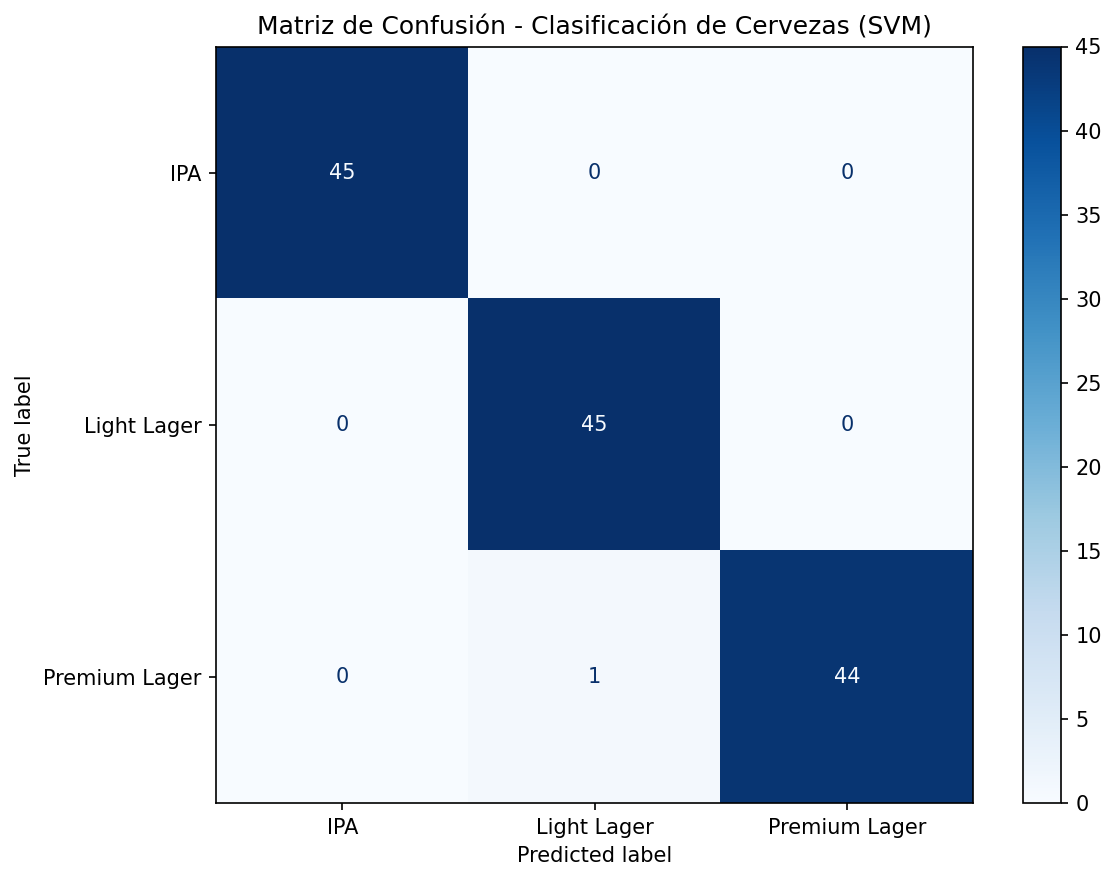
\includegraphics[width=0.6\textwidth]{images/p11.png}
    \caption{Matriz de confusión para la clasificación de cervezas con SVM.}
    \label{fig:p11}
\end{figure}

\subsection{Discusión}

El modelo SVM obtiene exactamente el mismo accuracy y F1-score que la red neuronal del Problema 5 (0.9926), clasificando incorrectamente solo una muestra de 135. La diferencia está en qué muestra se clasifica mal: mientras la NN confundió una IPA con Premium Lager, el SVM confundió una Premium Lager con Light Lager. Este último error es consistente con lo observado en la Tarea 2, donde los errores entre las dos variantes de Lager eran los más frecuentes por compartir características similares.

Este resultado confirma nuevamente que las cuatro features son altamente discriminativas para este problema y que prácticamente cualquier modelo de clasificación logra un desempeño excelente, independientemente del tipo de modelo utilizado.

\subsection{Conclusión}

SVM alcanza el mismo desempeño que la red neuronal (F1 = 0.9926) con solo 15 muestras de entrenamiento. Junto con los resultados de KNN en la Tarea 2, queda claro que este dataset presenta clases naturalmente bien separadas, haciendo que la elección del modelo sea menos relevante para el desempeño final.

% ========================================
% SECCIÓN 12
% ========================================
\section{Problema 12}

\subsection{Enunciado}

Repita el problema 6 utilizando el modelo SVM de sklearn. Anote los hiperparámetros que elija y todas sus suposiciones.

\subsection{Metodología}

\subsubsection{Generación y preprocesamiento de datos}

Se utiliza la misma generación de datos sintéticos del Problema 6: 3000 ecuaciones cuadráticas balanceadas en tres clases según el discriminante $\Delta = b^2 - 4ac$ (complejas, doble, reales distintas). Los coeficientes $(a, b, c) \in [-10, 10]$ con $|a| \geq 0.1$, y la clase de raíz doble se genera con perturbación $\pm 0.05$ alrededor de $c = b^2/(4a)$.

Se aplica normalizar con \texttt{StandardScaler} y se divide en 80\% entrenamiento (2400 muestras) y 20\% prueba (600 muestras) con estratificación, exactamente igual que en el Problema 6 para permitir una comparación directa.

\begin{lstlisting}
scaler = StandardScaler()
X_train_scaled = scaler.fit_transform(X_train)
X_test_scaled = scaler.transform(X_test)
\end{lstlisting}

\subsubsection{Configuración del modelo}

Se utiliza \texttt{SVC} con la misma configuración base de los Problemas 10 y 11 (clasificación con SVM). El objetivo es evaluar cómo se compara SVM contra NN y KNN en este problema donde la frontera de decisión está definida por la superficie cuadrática $\Delta = b^2 - 4ac = 0$.

\begin{lstlisting}
model = SVC(
    kernel='rbf',
    C=10,
    gamma='scale',
    random_state=14
)
\end{lstlisting}

\begin{itemize}
    \item \texttt{kernel='rbf'}: se mantiene el kernel gaussiano, esencial para este problema dado que la frontera de decisión ($\Delta = 0$) es una superficie cuadrática que no puede ser capturada por un kernel lineal.
    \item \texttt{C=10}: se mantiene consistente con los problemas de clasificación SVM anteriores (Problemas 10 y 11). Se experimentó con $C=100$ (el valor de los problemas de regresión SVM), pero la mejora fue marginal, probablemente porque con 2400 muestras de entrenamiento y solo 3 features, el riesgo de sobreajuste es bajo y el modelo ya encuentra buenos vectores de soporte con $C=10$.
    \item \texttt{gamma='scale'}: cálculo automático. Se intentó \texttt{gamma='auto'} ($\gamma = 1/n_{features} = 1/3$), pero \texttt{'scale'} produjo mejores resultados al considerar la varianza de los datos.
\end{itemize}

\subsection{Resultados}

\begin{table}[H]
\centering
\begin{tabular}{lcc}
\hline
& \textbf{Accuracy} & \textbf{F1 (weighted)} \\
\hline
Entrenamiento & 0.9383 & 0.9392 \\
Prueba        & 0.9417 & 0.9423 \\
\hline
\end{tabular}
\caption{Métricas de evaluación para la clasificación de raíces con SVM.}
\label{tab:p12_resultados}
\end{table}

\begin{table}[H]
\centering
\begin{tabular}{lcccc}
\hline
& \textbf{Precision} & \textbf{Recall} & \textbf{F1-score} & \textbf{Support} \\
\hline
Complejas ($\Delta<0$)   & 0.96 & 0.94 & 0.95 & 200 \\
Doble ($\Delta\approx0$) & 0.87 & 0.97 & 0.92 & 200 \\
Reales ($\Delta>0$)      & 1.00 & 0.92 & 0.96 & 200 \\
\hline
\end{tabular}
\caption{Reporte de clasificación detallado para el problema de raíces con SVM.}
\label{tab:p12_report}
\end{table}

\begin{figure}[H]
    \centering
    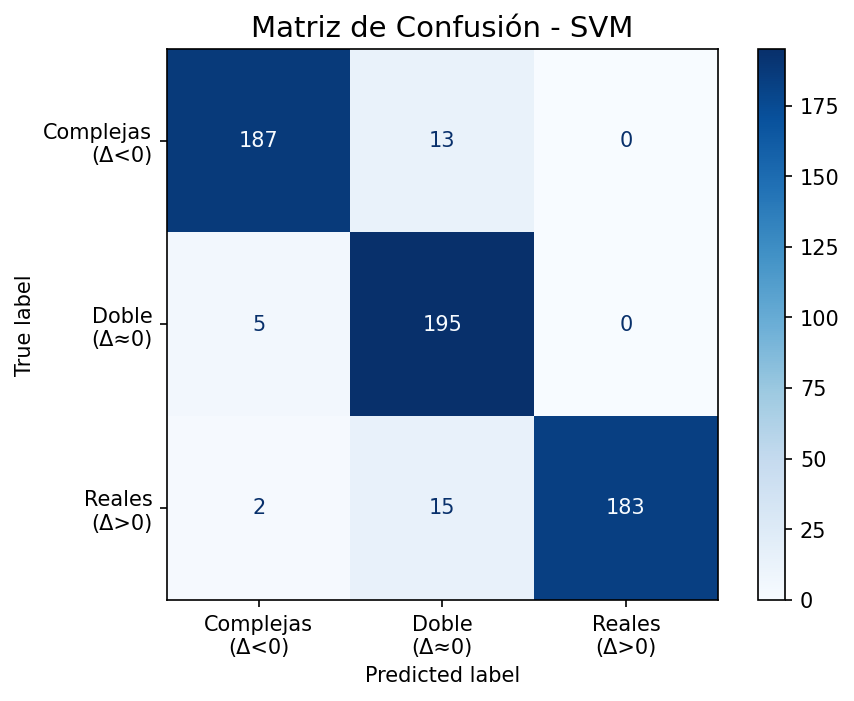
\includegraphics[width=0.6\textwidth]{images/p12.png}
    \caption{Matriz de confusión para la clasificación de raíces de ecuaciones cuadráticas con SVM.}
    \label{fig:p12}
\end{figure}

\subsection{Discusión}

El modelo SVM alcanza un accuracy de prueba de 0.9417, inferior al de la red neuronal del Problema 6 (0.9717). La clase de raíz doble ($\Delta \approx 0$) sigue siendo la más problemática, pero con una precision reducida a 0.87 (vs 0.94 en NN), lo que indica más falsos positivos: el SVM tiende a clasificar como raíz doble casos que en realidad son complejos o reales distintos.

\begin{table}[H]
\centering
\begin{tabular}{lcc}
\hline
\textbf{Modelo} & \textbf{Accuracy} & \textbf{F1 (weighted)} \\
\hline
KNN (T02, $k$=1)  & 0.8950 & 0.8954 \\
NN (P6)            & 0.9717 & 0.9718 \\
SVM (P12)          & 0.9417 & 0.9423 \\
\hline
\end{tabular}
\caption{Comparación de modelos para clasificación de raíces de ecuaciones cuadráticas.}
\label{tab:p12_comparacion}
\end{table}

La red neuronal fue el mejor modelo para este problema, seguida por SVM y luego KNN. Esto tiene sentido porque la frontera que separa los tipos de raíces depende de una relación no lineal entre los coeficientes, y la NN tiene mayor flexibilidad para aprender ese tipo de fronteras complejas.

Es notable que la accuracy de prueba de SVM (0.9417) es ligeramente superior a la de entrenamiento (0.9383), lo que indica que no hay sobreajuste y que el modelo podría beneficiarse de un valor de \texttt{C} más alto para un ajuste más preciso.

\subsection{Conclusión}

El modelo SVM logró un buen desempeño (accuracy 0.9417) en la clasificación de raíces cuadráticas, superando a KNN pero quedando por debajo de la red neuronal. La naturaleza no lineal de la frontera entre clases favorece a modelos más flexibles, y en este caso la NN demostró tener mayor capacidad para aprender esa frontera.

% ========================================
% SECCIÓN 13
% ========================================
\section{Problema 13}

\subsection{Enunciado}

Considere un modelo de clasificación. ¿Por qué el vector de parámetros $\theta$ es ortogonal a la frontera de decisión? Escriba su respuesta.

\subsection{Análisis}

Para responder esta pregunta conviene pensar en el caso más simple: un clasificador lineal. En este tipo de modelo, la predicción se hace combinando las características de entrada con los pesos del modelo ($\theta$) y sumando un sesgo. La frontera de decisión es la línea (o plano, en más dimensiones) donde el modelo no se inclina por ninguna clase.

Esa frontera se define por la ecuación $\theta^T x + b = 0$. Si tomamos dos puntos cualesquiera sobre la frontera y los restamos, el sesgo se cancela y lo que queda es que la diferencia entre esos puntos es perpendicular a $\theta$. Como esa diferencia representa cualquier dirección posible dentro de la frontera, se concluye que $\theta$ es perpendicular a toda la frontera.

Dicho de forma más intuitiva: $\theta$ apunta en la dirección donde el modelo más distingue entre clases. Si caminamos en esa dirección, cruzamos la frontera rápidamente y pasamos de una clase a otra. En cambio, si caminamos a lo largo de la frontera, la salida del modelo no cambia en absoluto, que es justamente lo que significa ser ortogonal.

Esta propiedad no aplica solo a clasificadores lineales simples. En regresión logística y en SVM funciona de la misma manera: el vector de pesos siempre apunta en la dirección perpendicular a la frontera de decisión. De hecho, en los problemas 10, 11 y 12 de esta tarea se usó SVM para clasificación, y en todos esos casos el modelo encontró fronteras que separan las clases con el vector de pesos perpendicular a ellas.

\subsection{Conclusión}

En resumen, $\theta$ es ortogonal a la frontera de decisión porque la frontera es el lugar donde la combinación $\theta^T x + b$ vale cero, y moverse dentro de ella no cambia la salida del modelo. La dirección de $\theta$ es justamente la que cruza la frontera, separando una clase de otra.

% ========================================
% REFERENCIAS
% ========================================
\bibliographystyle{plainurl}
\bibliography{ref}


\end{document}